\begin{problem} {Rod-Cutting}
    Given a rod of length n inches and a
table of prices pi for i= 1,2,3...i determine the maximum revenue obtainable by cutting up the rod and selling the pieces. Note that if the price pn for a rod
of length n is large enough, an optimal solution may require no cutting at all.
\end{problem}

\marginnote{
    MarginNotes
}

\begin{solution}
    (1)
    \vspace{3mm}
    \hrule
    
    \begin{intution}
        Similarity to unbounded knapsack if we consider the solution array(sarr) derived from cost[].
    \end{intution}

        % 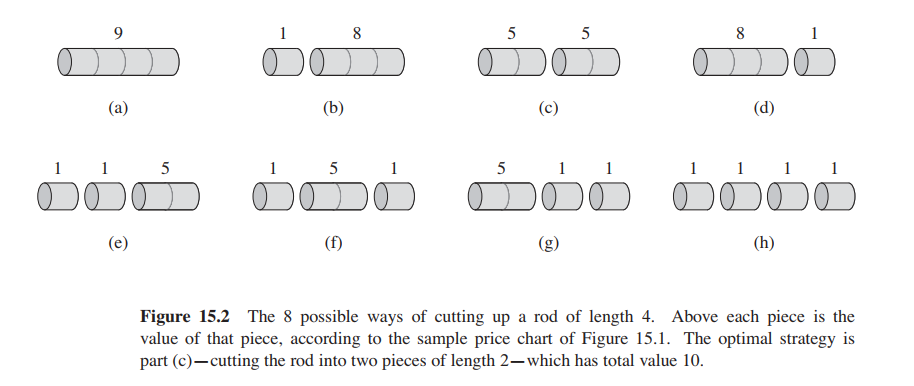
\includegraphics[width=10cm, height=5cm]{./diagram/rod-cutting-example.png}
        
       Considering the cost[], we will try to find sarr[]. \\
       where sarr[idx] := maximum revenue we can get if we are allowed to cut rod from length cost[0..idx-1]
       Now, for the sarr[] at index idx.
       We have two options:
        \begin{enumerate}[(a)]
            \item get the profit arr[idx] $\Rightarrow$ we can again cut the reduced rod with profit arr[idx] $val1 = cost[idx] + f(idx,n-(idx+1))$
            \item do not get the profit arr[idx] $val2 = f(idx+1,n)$
        \end{enumerate}
    \begin{verbatim}
        int findAns(int idx,int n ,const vector<int>& arr)
        {
            if(idx >= arr.size()) return 0;
            
            int val1 = INF; //inclusive : keep getting profit arr[idx] if its possible
            
            int val2 = INF; //exclusive: do not get profit arr[idx]
            
            int cut_length = idx+1;
            if(n-cut_length>=0)
                val1 = arr[idx] + findAns(idx,n-cut_length,arr); //rod-lenght is reduced
                
            val2 = findAns(idx+1,n,arr); 
            
            printf("[%d,%d]: (%d,%d)\n",idx,n,val1,val2);
            return max(val1,val2);
        }
    \end{verbatim}
\end{solution}


\begin{solution}
    (2)
    \vspace{3mm}
    \hrule
    
    \begin{intution}
        Consider the function signature as :
        $f(n) :=$ maximum revenu we can make if we have a rod of lenght n
    \end{intution}

    If we have rod of lenght n, that we can do cost.size() number of operations on this rod. (i.e we will try to cut this at all possible place)

    \begin{verbatim}
        int findAnsTwo(int n,const vector<int>& arr)
        {
            if(n<=0) return 0;
            int &mans = memt[n];
            if(mans != -1) return mans;

            int profit = INF;
            /* try to cut the rod in all possible way := cut the rod at 1,
            cut the rod at 2, ...
            */
            for(int k=1;k<=n;k++) //
            {
                int tprofit = arr[k-1] + findAnsTwo(n-k,arr); 
                /* question has 1 based index , so we do arr[k-1]*/
                profit = max(profit,tprofit);
            }

            return mans = profit;
        }
    \end{verbatim}
    
\end{solution}

% sol_file: /code/rod-cutting.cpp